\newpage
\chapter{Process description}
\mbox{}\vspace{-\baselineskip}
\label{Chap:kin}

\section{Process kinematics}




Figure~\ref{fig:diagram} introduces the process that is proposed to be investigated to study color transparency effects in the NICA SPD experiment, i.e., left side of Fig.~\ref{fig:diagram} shows the diagram of the hard proton knock-out from a deuteron in $p-d$ collisions, while its right side sketches the same process but for the case of $d-d$ collisions. For the latter, the neutron $p_{s_{1}}$ of the deuteron $d_{1}$ is assumed to be quasi-free, meaning that no rescatterings of other participating nucleons off the neutron $p_{s_{1}}$ take place and hence it remains a spectator to the whole $pd\rightarrow ppn$ process. Both diagrams represent impulse approximation (IA) part of the process $pd\rightarrow ppn$, meaning that soft rescatterings of the protons $p_{1}$, $p_{3}$ and $p_{4}$ off the reaction neutron $p_{s}$ are not shown. For more details on the process formalism see Appendix~\ref{app_formalism}.



\begin{figure}[htp]
\begin{center}
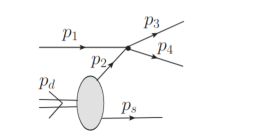
\includegraphics[width=8.2cm]{pictures/diagram.pdf}
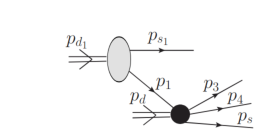
\includegraphics[width=8.2cm]{pictures/diagram2.pdf}
\caption{\small  Impulse approximation (IA) diagrams for the process $pd\rightarrow ppn$ (left) and the process $dd\rightarrow ppnn$ (right). For both diagrams, the following notations are used for the particles' four-momenta: $p_{d}$ and $p_{d_1}$ correspond to the deuterons in the initial state, $p_{1}$ -- the incoming/initial proton, $p_{2}$ -- the intermediate/reaction proton (not shown in the right diagram), $p_{s}$ and $p_{s_1}$ -- the final state neutrons, and $p_{3}$ and $p_{4}$ -- the final state protons.} \label{fig:diagram}
\end{center}
\end{figure}

\newpage

In the center-of-mass system of the two colliding deuterons $d$ and $d_{1}$ with the $z$-axis pointing along the momentum of $d_{1}$ (which is the same as the Lab system), the deuteron four-momenta are given by
\begin{equation}
\begin{aligned}
&P_{d1}^{\mu} &=&~~(0,~~~0,~~~\sqrt{s/4-m_{d}^{2}},~~\sqrt{s}/2)~~~\textrm{and}\\
&P_{d}^{\mu} &=&~~(0,~~~0,~-\sqrt{s/4-m_{d}^{2}},~~\sqrt{s}/2 ),\\
\end{aligned}\label{eq:deuteron_mom}
\end{equation}
where $\sqrt{s}$ is the invariant mass (energy) of the colliding deuterons and $m_{d}$ is the deuteron~mass. 

For the process introduced in Fig.~\ref{fig:diagram}, energy-momentum conservation compels the four-momenta of the participating particles to satisfy the following relations. 
\begin{equation}
\enspace \enspace \enspace  \enspace \enspace\left( P_{1}^{\mu}+P_{2}^{\mu} \right)^2 =~~\left( P_{3}^{\mu}+P_{4}^{\mu} \right)^2.\\
\label{eq:momenta1}
\end{equation}
\begin{equation}
~~~\left( P_{3}^{\mu}+P_{4}^{\mu}+P_{s}^{\mu} -P_{d}^{\mu} \right)^2 =~~~~~~\left(P_{1}^{\mu} \right)^2~~~~ =~~m_{p}^{2}.\\
\label{eq:momenta2}
\end{equation}
\begin{equation}
\left( P_{3}^{\mu}+P_{4}^{\mu}+P_{s}^{\mu} + P_{s_{1}}^{\mu} \right)^2 =~~\left( P_{d_{1}}^{\mu}+P_{d}^{\mu} \right)^2=~~s.\\
\label{eq:momenta3}
\end{equation}




Here $P_{i}^{\mu}$ are the four-momenta of the particle $i$ and $m_{p}$ is the proton rest mass. Note~that soft rescatterings of the protons off both neutrons $p_{s}$ and $p_{s1}$ introduce distortions into Eq.~\eqref{eq:momenta1}. In turn, Eq.~\eqref{eq:momenta2} acquires distortions only due to interactions with the neutron $p_{s1}$ but is not affected by interactions with the neutron $p_{s}$. Finally, Eq.~\eqref{eq:momenta3} is not affected by soft rescatterings off either neutrons (as long as no new particles are produced). For the protons $p_{1}$ and $p_{2}$ in the initial state, note that (i) they are assumed to be on-shell and (ii) in the rest frame of the corresponding deuterons, they move with the Fermi momentum.



Provided that in the proposed experiment, the reaction final particles are detected and their four-momenta are known, the relations in Eqs.~\eqref{eq:momenta1}~\eqref{eq:momenta2},~and~\eqref{eq:momenta3} can be used in the data analysis to separate the events of interest from all other registered events and to isolate the desired reaction (see more details in Sec.~\ref{sec:topologies}). Also note that (if used in the data analysis) Eq.~\eqref{eq:momenta1} will be subject to the Fermi-smearing due to the fact that the Fermi momenta of the protons $p_{1}$ and $p_{2}$ will not be experimentally accessible. 



\section{Kinematic variables}

Figure~\ref{fig:kin_planes} shows the kinematics of the process $pd\rightarrow ppn$ in the rest frame of the deuteron $d$ with the $z$-axis pointing along the momentum of the incoming proton $p_{1}$ (particle notations are the same as in Fig.~\ref{fig:diagram}).

The process $pd\rightarrow ppn$ is described by four independent variables. As suggested in Ref.~\cite{PhysRevC.107.014605}, the convenient choice of the kinematic variables is the following, $\alpha_s$, $p_{st}$, $t$, and $\phi$, which are defined in the rest frame\footnote[1]{To boost to the deuteron rest frame, $\beta=-\sqrt{1-\frac{4m_{d}^2}{s}}$.} of the deuteron $d$ (see Figs.~\ref{fig:diagram} and~\ref{fig:kin_planes}). The variables are described below in more detail.

\begin{itemize}

\item  \mbox{\large$\alpha_{s}=\frac{2(E_{s}-p_{sz})}{m_{d}}$} is the light cone variable that is convenient for the description of high energy processes. Here $E_{s}$ and $p_{sz}=\left| \overrightarrow{p_{s}}\right|\textrm{cos}\angle \left(\overrightarrow{p_{1}}, \overrightarrow{p_{s}} \right)$ are the energy of the spectator neutron and its longitudinal momentum with respect to the incoming proton momentum $p_{1}$, respectively. 

\item $p_{st}$ is the transverse momentum of the spectator neutron ($p_{s}$) with respect to the incoming proton momentum ($p_{1}$). The variable $p_{st}$ is defined as follows, given that $\overrightarrow{p_{s}}$ and $\overrightarrow{p_{1}}$ are the three-momenta of the particles $p_{s}$ and $p_{1}$, respectively.
\begin{equation}
p_{st} = \sqrt {\left| \overrightarrow{p_{s}} \right|^{2} -  \frac{\left( \overrightarrow{p_{1}}\cdot \overrightarrow{p_{s}}\right)^{2}}{\left| \overrightarrow{p_{1}} \right|^{2}}} = \left| \overrightarrow{p_{s}} \right| \sqrt{1-\textrm{cos}^{2}\angle \left(\overrightarrow{p_{1}}, \overrightarrow{p_{s}} \right)} = \left| \overrightarrow{p_{s}}\right|\textrm{sin}\angle \left(\overrightarrow{p_{1}}, \overrightarrow{p_{s}} \right) .\label{eq:cyy}
\end{equation}

\item $t=\left(P^{\mu}_{1}-P^{\mu}_{3}\right)^{2}$ is the Mandelstam variable with $P^{\mu}_{1}$ and $P^{\mu}_{3}$ being the four-momenta of the incoming and scattered protons, respectively.  Note also that $Q^{2} = -t = \frac{1}{2}\left [s_{34}-4m^{2}\right ]\left [1-\textrm{cos}(\theta_{\textrm{c.m.}})\right ]$, where $s_{34} = \left(P^{\mu}_{3}+P^{\mu}_{4}\right)^{2}$ is the invariant mass of the final protons and $P^{\mu}_{3}$ and $P^{\mu}_{4}$ are the proton four-momenta, $m$ the nucleon mass, and $\theta_{\textrm{c.m.}}$ is the polar angle of the scattered proton $p_{3}$ in the center-of-mass frame of the colliding deuterons with the $z$-axis pointing along the direction of the $d_{1}$ (which is the same as the Lab frame).

\item $\phi = \phi_{3}-\phi_{s}$ is the relative azimuthal angle between the scattered proton and the spectator neutron (i.e. between the ($p_{1}$,~$p_{3}$) and ($p_{1}$, $p_{s}$) planes in Fig.~\ref{fig:kin_planes}).

\end{itemize}



\begin{figure}[htp]
\begin{center}
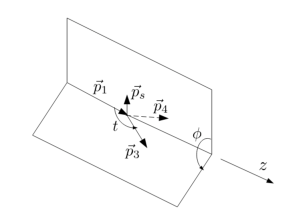
\includegraphics[width=8.2cm]{pictures/kin_planes.pdf}
\caption{\small Kinematics of the process $pd\rightarrow ppn$ in the rest frame of the deuteron $d$ with the $z$-axis pointing along the momentum of the incoming proton $p_{1}$. Notations for the particles' four-momenta are the same as in Fig.~\ref{fig:diagram}. Kinematic variables $\phi$ and $t$ are described in the text.} \label{fig:kin_planes}
\end{center}
\end{figure}

\newpage

As derived in Ref.~\cite{PhysRevC.107.014605}, the four-differential cross section of the process $pd\rightarrow ppn$ takes the following form with all the involved variables described above.
{\normalsize
\begin{equation}
 \frac{\alpha_{\textrm{s}}}{p_{\textrm{st}}}\frac{\textrm{d}^{4}\sigma}{\textrm{d}p_{\textrm{st}}\textrm{d}\alpha_{s}\textrm{d}t \textrm{d}\phi }.\label{eq:cr_sect}
\end{equation}
}

As shown in Ref.~\cite{Larionov:2025equ}, for the process $dd\rightarrow ppnn$, the cross section in Eq.~\eqref{eq:cr_sect} should also be divided by the factor that corresponds to the integral of the wave function of the deuteron $d_{1}$ (which will be different from unity if cuts are imposed on the $d_{1}$ momentum).

It is also important that all kinematic variables for the process $pd\rightarrow ppn$ are defined with respect to the incoming proton $p_{1}$, and therefore, information on the $p_{1}$ actual momentum is required (for each reaction event) to correctly calculate the variables. However, since the $p_{1}$ momentum is convoluted with the Fermi momentum, it is unlikely that this information will be experimentally accessible. As a standard compromise for deuteron experiments~\cite{CLAS:2023mfc,my_an_note:2020,my_thesis:2021,Skorodumina:2015rea, CLAS:2022kta,note_mm_distr}, the kinematic variables can be calculated assuming that the proton $p_{1}$ has no Fermi momentum and moves in the direction of the deuteron $d_{1}$. This assumption will lead~to~the Fermi-smearing of the kinematic variables (and the cross sections binned in them). In general, there are two ways in which this issue can be dealt with, i.e. (i) the Fermi smeared cross sections can be extracted and then analyzed within the model to estimate the CT contribution, meaning that the model itself has to account for the cross section Fermi-smearing or (ii) a special ``unfolding" correction can be developed based on the Monte-Carlo simulation to retrieve the unsmeared cross-section (as was done e.g. in the study in Refs.~\cite{CLAS:2023mfc,my_an_note:2020,my_thesis:2021}).





